\section{Experiments}
\label{sec:experiments}
In this section, we study {\sys} on nine workloads and three host engines. We test its gains over the host and existing rewriters~(Section~\ref{sec:exp:e2e}), as data and concurrency grow~(Section~\ref{sec:exp:scalability}), and on queries its rules were not distilled from~(Section~\ref{sec:exp:generalization}). We also measure the cost to specialize~(Section~\ref{sec:exp:generation}) and correctness (Section~\ref{sec:exp:verification}), and discuss the impact of rule ordering and the host engine (Section~\ref{sec:exp:discussion}).

% TODO(Saeed): fill the \blue{?} cells in tables/datasets.tex (Stats row, IMDB Full sample size, DSB 52 or 53, coverage, CEB rule source).
\begin{table}[!t]
% \vspace{-0.1cm}
    \centering
    \caption{Datasets and Workloads: Sample Size $|\mathcal{Q}_s|$ for Rule Generation, Rules Generated, and Coverage (\% of Queries and \% of Host Time Where at Least One Rule Fires).}
    \vspace{-0.4cm}
    \label{tbl:datasets}
    \resizebox{0.99\columnwidth}{!}{
        \small \setlength\tabcolsep{3pt}
        \begin{tabular}{llrrrr}
        \toprule
        \textbf{Dataset (\# Tables)} & \textbf{Workload} & \textbf{\# Queries} & $|\mathcal{Q}_s|$ & \textbf{\# Rules} & \textbf{Coverage} \\ \midrule
        TPC-H, sf=100 (8)           & TPC-H         & 22                 & 5                   & 12            & 50.0\,/\,39.0 \\
        DSB, sf=100 (25)            & DSB           & 52                 & 11                  & 25            & 94.3\,/\,99.1 \\
        Stats-CEB (8)               & Stats-CEB     & 146                & 5                   & 16            & 100\,/\,100 \\
        Stats (8)                   & Stats         & 146                & 0                   & 16$^\dagger$  & 100\,/\,100 \\        
        IMDB (21)                   & JOB           & 113                & 6                   & 19            & 100\,/\,100 \\
                                    & JOB-Complex   & 30                 & 5                   & 18            & 100\,/\,100 \\
                                    & IMDB Full     & 13,646             & 5                   & 23            & 100\,/\,100 \\
                                    & CEB, sf=1--10 & 16                 & 0                   & 67$^\dagger$  & 100\,/\,100 \\
        StackOverflow, sf=1\,\&\,12 (8) & SQLStorm  & 1,190              & 8                   & 12            & 100\,/\,100 \\
                                    & SQLStorm (full) & 18,251           & 8                   & 12$^\dagger$  & 69.1\,/\,65.3 \\
        \midrule
        \multicolumn{4}{l}{Total (distinct after deduplication)} & 125 (67) & \\
        \bottomrule
    \end{tabular}
}
\vspace{-0.1cm}
\raggedright\footnotesize $^\dagger$\,No LLM call, not counted in the total: \textsf{Stats} reuses the 16 \textsf{Stats-CEB} rules (same queries, different data); \textsf{CEB} applies the pooled library.
\vspace{-0.45cm}
\end{table}

% \begin{table}[!t]
%     \centering
%     \caption{Used Datasets and their Workload Characteristics.}
%     \vspace{-0.4cm} 
%     \label{tbl:datasets}
%     \resizebox{0.99\columnwidth}{!}{
% 		\small \setlength\tabcolsep{0.2pt}
%         %\addtolength{\tabcolsep}{.5em}	
%         \begin{tabular}{cccc}
%         \toprule
%         \textbf{Dataset}   & \textbf{\# Tables} & \textbf{Workload (\# Queries)}             \\ \midrule 
%         TPC-H (sf=100)     & 8                  & TPC-H (22)                         \\
%         Stats(-ceb)        & 8                  & 146                                        \\
% 				IMDB               & 21                 & JOB (113), Full (13,646), JOB-Complex (30), CEB (16) \\                  
%         StackOverflow (sf=1 \& 12)      & 8                  & SQLStorm (18,251, 1,190)                          \\
%         DSB (sf=100)       & 25                 & DSB (52)                           \\
%         \bottomrule
%     \end{tabular}
% }
% \vspace{-0.35cm}  
% \end{table}


\begin{figure*}[!t]
      \centering
    
\includegraphics[scale=0.5]{plots/Experiment2-EtoE-Overview-Legend-1}\vspace{-0.2cm}

    \subfigure[\label{fig:overall_1pg}PostgreSQL]{
        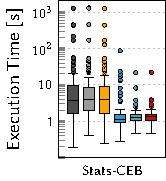
\includegraphics[scale=0.79]{plots/Experiment1-STATS-CEB-PG-EtoE}
        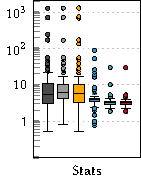
\includegraphics[scale=0.79]{plots/Experiment1-STATS-PG-EtoE}
        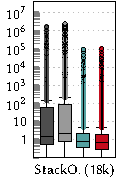
\includegraphics[scale=0.79]{plots/Experiment1-Stackoverflow_18k-PG-EtoE}
    }
    
\includegraphics[scale=0.45]{figures/img/fig_delimiter}
    \subfigure[\label{fig:overall_1mysql}MySQL]{
        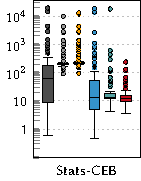
\includegraphics[scale=0.79]{plots/Experiment1-STATS-CEB-MySQL-EtoE}
        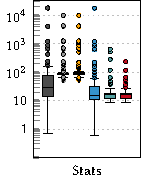
\includegraphics[scale=0.79]{plots/Experiment1-STATS-MySQL-EtoE}
        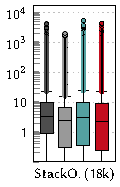
\includegraphics[scale=0.79]{plots/Experiment1-Stackoverflow_18k-MySQL-EtoE}
    }
 
\includegraphics[scale=0.45]{figures/img/fig_delimiter}
    \subfigure[\label{fig:overall_1duckdb}DuckDB]{
        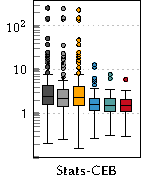
\includegraphics[scale=0.79]{plots/Experiment1-STATS-CEB-DuckDB-EtoE}
        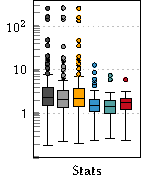
\includegraphics[scale=0.79]{plots/Experiment1-STATS-DuckDB-EtoE}
        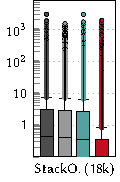
\includegraphics[scale=0.79]{plots/Experiment1-Stackoverflow_18k-DuckDB-EtoE}
    }

    \vspace{-0.55cm}
    \caption{Per-query Execution Time on Three Datasets and Three Engines: {\sys} Removes the Slow Outliers That Dominate Workload Time, While Medians Change Little. ReSequel and R-Bot Were Not Run on StackOverflow (18k).}
    \label{fig:overall_1}
    \vspace{-0.3cm}
\end{figure*}

% TODO(Saeed): fill every \blue{?} cell from existing logs (host time, ReSequel and SOLEX speedups).
%   Use "--" where a system was not run. Add the host time for CEB (scale factors 1 and 10).
% MB: please also make the best speedup per workload and system bold, second best underline
% Saeed: The LLM-R2 results were missing from the new outline, so I added both LLM-R2 and R-Bot for PostgreSQL. 
\begin{table*}[!t]
\centering
\small \setlength\tabcolsep{4.6pt}
\caption{Host Workload Time and Speedup ($\times$) of \blue{LLM-based} Rewriters and {\sys}. \textbf{Bold}: Best, \underline{Underline}: Second, ``--'': Not Run.}
\label{tbl:e2e}
\vspace{-0.4cm}
\resizebox{.99\textwidth}{!}{
\begin{tabular}{l|rrrrr|rrr|rrr}
\toprule
 & \multicolumn{5}{c|}{\textbf{PostgreSQL}} & \multicolumn{3}{c|}{\textbf{MySQL}} & \multicolumn{3}{c}{\textbf{DuckDB}} \\
\textbf{Workload} & Host & LLM-R2 & R-Bot & ReSequel & {\sys} & Host & ReSequel & {\sys} & Host & ReSequel & {\sys} \\
\midrule
\textsf{TPC-H} (22) & $40.2$\,h & $\mathbf{1.36}\times$ & $0.38\times$ & \underline{$1.11\times$} & $1.03\times$ & $115.8$\,h & \underline{$1.18\times$} & $\mathbf{1.69}\times$ & $900.4$\,s & \underline{$0.93\times$} & $\mathbf{1.11}\times$ \\
\textsf{DSB} (52) & $113.4$\,h & $2.37\times$ & $0.39\times$ & \underline{$7.45\times$} & $\mathbf{7.71}\times$ & $42.4$\,h & \underline{$6.27\times$} & $\mathbf{6.96}\times$ & $800.1$\,s & $\mathbf{1.23}\times$ & \underline{$0.89\times$} \\
\textsf{Stats} (146) & $3{,}782.6$\,s & -- & $1.02\times$ & \underline{$10.9\times$} & $\mathbf{26.9}\times$ & $9.7$\,h & \underline{$1.39\times$} & $\mathbf{29.2}\times$ & $933.8$\,s & \underline{$8.92\times$} & $\mathbf{11.3}\times$ \\
\textsf{Stats-CEB} (146) & $3{,}135.6$\,s & -- & $1.03\times$ & \underline{$12.9\times$} & $\mathbf{38.7}\times$ & $22.0$\,h & \underline{$1.8\times$} & $\mathbf{60.5}\times$ & $952.0$\,s & \underline{$8.5\times$} & $\mathbf{11.6}\times$ \\
\textsf{JOB} (113) & $4{,}808.3$\,s & \underline{$1.02\times$} & $0.11\times$ & $0.97\times$ & $\mathbf{1.07}\times$ & $3.0$\,h & \underline{$1.07\times$} & $\mathbf{1.42}\times$ & $277.1$\,s & $\underline{1.03}\times$ & $\mathbf{1.26}\times$ \\
\textsf{JOB-Complex} (30) & $1{,}076.1$\,s & -- & $0.002\times$ & $\mathbf{4.53}\times$ & \underline{$3.73\times$} & $90.7$\,h & \underline{$0.71\times$} & $\mathbf{5.85}\times$ & $142.0$\,s & \underline{$0.94\times$} & $\mathbf{1.04}\times$ \\
\textsf{IMDB Full} (13,646) & $97.0$\,h & -- & -- & \underline{$0.84\times$} & $\mathbf{1.66}\times$ & -- & -- & -- & $6.3$\,h & \underline{$1.29\times$} & $\mathbf{1.44}\times$ \\
\textsf{StackOverflow} SF\,1 (1,190) & $749.7$\,s & -- & -- & $\mathbf{1.90}\times$ & \underline{$1.82\times$} & $5{,}815.3$\,s & $\mathbf{4.19}\times$ & \underline{$3.62\times$} & $663.8$\,s & \underline{$1.02\times$} & $\mathbf{1.64}\times$ \\
\textsf{StackOverflow} SF\,12 (1,190) & $5.5$\,h & -- & -- & \underline{$2.45\times$} & $\mathbf{2.92}\times$ & $31.7$\,h & \underline{$4.26\times$} & $\mathbf{12.58}\times$ & $5{,}666.7$\,s & \underline{$0.99\times$} & $\mathbf{1.67}\times$ \\
\textsf{StackOverflow} (18,251) & $8{,}849.6$\,h & -- & -- & -- & $4.47\times$ & $438.2$\,h & -- & $1.02\times$ & $96.4$\,h & -- & $1.43\times$ \\
\midrule
\textsf{Stats-CEB}, \textsf{JOB} rules & $3{,}135.6$\,s & -- & -- & -- & $28.3\times$ & $22.0$\,h & -- & $6.6\times$ & $952.0$\,s & -- & $9.8\times$ \\
\textsf{CEB} (16), SF\,1--10 & -- & -- & -- & -- & -- & -- & -- & -- & $5{,}022$--$6{,}401$\,s & -- & $31.4$--$200\times$ \\
\bottomrule
\end{tabular}
}
\vspace{-0.15cm}
\end{table*}

\subsection{Experimental Setup}
\label{sec:exp:setup}

\textbf{Implementation:} {\sys}'s rewriting engine is implemented in C++17; LLM inference and communication in Python. The parser and unparser are built on DuckDB's parser~\cite{DuckDB} with broad SQL coverage. To emit dialect-specific SQL, we implement unparsing rules from DuckDB's internal representation to the target dialect, with support for PostgreSQL, MySQL, and DuckDB. Rewrite rules are compiled to native shared libraries and loaded at runtime via \texttt{dlopen} (Section~\ref{sec:offline:implement}). Offline rule generation uses ReSequel~\cite{resequel} as LLM rewriter with Gemini-3.1-pro~\cite{gemini}.
Each rule passes the verification of Section~\ref{sec:offline:verify}: a smoke test, a formal check with SQLSolver~\cite{SQLSolver}, and a result-equivalence test on sampled data if needed.

\textbf{Benchmarks:} Table~\ref{tbl:datasets} summarizes the datasets and their workloads, which range from small synthetic benchmarks to large real-world corpora. \textsf{TPC-H}~\cite{tpch} and \textsf{DSB}~\cite{DSB} are synthetic OLAP benchmarks, while \textsf{Stats} and \textsf{Stats-CEB}~\cite{CEDBMS} cover real-world StackExchange analytics. \textsf{JOB}~\cite{LeisGMBK015}, \textsf{IMDB Full}~\cite{flowloss}, and \textsf{JOB-Complex}~\cite{JOBComplex} exercise complex multi-join plans over the \textsf{IMDB} schema, the last a join-intensive benchmark. \textsf{StackOverflow}~\cite{SQlStorm} is a large-scale LLM-generated workload over a real-world schema.

\textbf{Hardware and Software:} All experiments run on a VM with Intel CPU (32~vCPUs) and 148~GB DDR4 RAM, Ubuntu~22.04, C++17, PostgreSQL~18.3, MySQL~8.0.46, and DuckDB~1.5.3. PostgreSQL is tuned with PGTune~\cite{PGTune} for OLAP workloads, MySQL's InnoDB buffer pool is set to 100~GB, and DuckDB requires no special tuning. All DBMSs run with multi-threading enabled.


% TODO(Saeed): confirm IMDB Full's sample: all 13,646 queries or its 79 templates?
% Saeed: Table and text update based on workload and samples
\textbf{Workload Samples:} {\sys} distills rules from a sample $\mathcal{Q}_s$ of each workload (Section~\ref{sec:offline:sample}). \blue{$\mathcal{Q}_s$ is the smallest query set covering all rules of a workload: 5 each for \textsf{TPC-H}, \textsf{Stats-CEB}, \textsf{JOB-Complex}, and \textsf{IMDB Full}, 6 for \textsf{JOB}, and 11 for \textsf{DSB}. On \textsf{StackOverflow}, $\mathcal{Q}_s$ has 8 of the 1,190 queries, and the rules run on all 18,251.} \blue{All rules are pooled into a library of 67 distinct rules. Section~\ref{sec:exp:e2e} reports results with this library, and Section~\ref{sec:exp:generalization} the generalization results when one workload's rules alone run on another.}

\textbf{Baselines:} We compare with the following strong \emph{query rewriting} baselines:
(1)~\emph{Host DBMS}: unmodified query execution on PostgreSQL, DuckDB, or MySQL;
(2)~\emph{ReSequel}~\cite{resequel}: LLM-based rewriter (Gemini-3.1-pro) that rewrites each query template with the LLM and serves cached rewrites to later queries of the same template;
(3)~\emph{LLM-R2}~\cite{LLMR2}: per-query LLM rewriter requiring query plan access; it needs workload-specific training, so we evaluate it only on the workloads of its publication;
(4)~\emph{R-Bot}~\cite{RBot}: rule-guided LLM rewriter;
(5)~\emph{LearnedRewrite}~\cite{learnedrewrite}: cost-model-guided rewriter using MCTS over Calcite rules.
We also compare against \emph{BespokeOLAP}~\cite{bespokeolap}, an LLM-synthesized engine, on \textsf{CEB} (Section~\ref{sec:exp:scalability}).
To evaluate the offline \emph{rule verification} step, we run three standalone verifiers: \emph{SQLSolver}~\cite{SQLSolver}, an SMT-based equivalence prover that encodes SQL semantics into linear integer arithmetic; \emph{QED}~\cite{QED}, an equivalence decider with broader SQL coverage (e.g., bags, \texttt{NULL}s, and integrity constraints); as well as \emph{VeriEQL}~\cite{VeriEQL}, a \emph{bounded} verifier that checks equivalence up to a fixed input size and returns a counterexample when a pair is non-equivalent.


\subsection{End-to-End Workload Performance}
\label{sec:exp:e2e}
This experiment tests whether {\sys}'s rules speed up workloads beyond what the host and existing rewriters achieve. Table~\ref{tbl:e2e} reports total runtime time per workload and engine. Figure~\ref{fig:overall_1} shows the per-query distributions on \textsf{Stats-CEB}, \textsf{Stats}, and \textsf{StackOverflow}.

\textbf{Source of Speedups:} Most queries change little, but the slowest ones speed up substantially and dominate the workload runtime. On DuckDB, \textsf{Stats-CEB} drops from $952.0$\,s to $82.2$\,s ($11.6\times$), with four queries accounting for $68\%$ of the saving. The largest is \textsf{query58}, a \texttt{COUNT(*)} star join that {\sys} factorizes into pre-aggregated CTEs, cutting it from $253.9$\,s to $354$\,ms ($717\times$); on PostgreSQL the same query drops from $1{,}278.5$\,s to $181$\,ms. The losses are small: $77$ of the $146$ queries run slower, but all of them finish in under $1.4$\,s and together they add $17.2$\,s, $1.8\%$ of the total. %, against $869.8$\,s saved.

\red{\textbf{Beyond Factorization:} Factorized aggregation is not the only high-impact rewrite {\sys} discovers. The other large gains come from three further rewrite classes, each of which a host optimizer lacks on at least one engine (Section~\ref{sec:background}). (1)~\emph{Decorrelation of scalar subqueries:} PostgreSQL evaluates a correlated scalar subquery as a per-row subplan; {\sys} rewrites it into a pre-aggregated CTE joined once. On \textsf{DSB}, this reduces \textsf{query081} from $71.3$\,h to $8.4$\,min ($504\times$), and a variant for correlations across different keys reduces \textsf{query032} from $27.4$\,h to $1.03$\,h ($26.5\times$); together, these two queries account for $99.9\%$ of the time saved on \textsf{DSB}. (2)~\emph{Eager aggregation:} on \textsf{DSB} \textsf{query025}, {\sys} groups \texttt{catalog\_sales} on its join keys before a many-to-many join and compensates the remaining sums with the group count, a $17\times$ speedup on PostgreSQL. (3)~\emph{Semijoin pre-filtering:} on \textsf{JOB-Complex}, {\sys} intersects the strongly filtered join branches into a key set and joins the hub table only on that set, which also brings the remaining join under PostgreSQL's join-reordering limit; \textsf{q23} runs $19.8\times$ faster. None of these rules is specific to its source query: each fires on its structural pattern, independent of tables and constants.}

\begin{figure*}[!t]
    \vspace{-0.15cm}
    \centering
    \resizebox{.98\textwidth}{!}{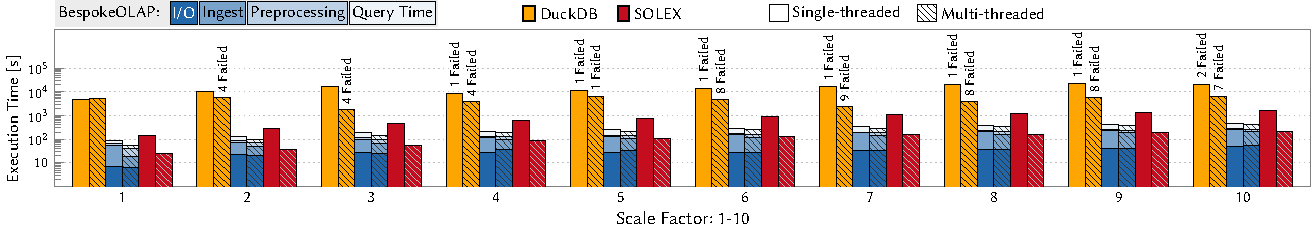
\includegraphics[scale=1]{plots/Experiment0-Micro-CEB}}
    \vspace{-0.45cm}
    \caption{\textsf{CEB} at Scale Factors 1--10, Single- and Multi-threaded (32 Threads): BespokeOLAP (Stacked by Phase) Wins Only Single-threaded, at \$303 of Synthesis Redone per Workload Change, and Gains Little from Threads as Preparation Dominates; {\sys} on DuckDB Gains Most by Reusing the Host's Parallel Engine; Labels Count DuckDB's Failed Queries.}
    % TODO(Saeed): rename ROLEX -> SOLEX in the plot legend.
    \label{fig:ceb_micro0}
    \vspace{-0.35cm}
\end{figure*}

% TODO(Saeed): regenerate this figure (plots/Experiment2-Stackoverflow*-Speed-Micro) with the old panel (c) only, sized for one column.
\begin{figure}[!t]
    \centering
     
\includegraphics[scale=0.47]{plots/Experiment2-Micro-Speed-Legend-2}\vspace{-0.05cm}\\
     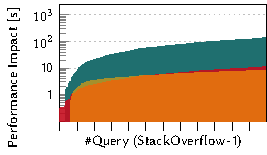
\includegraphics[scale=0.95]{plots/Experiment2-Stackoverflow1-Speed-Micro}
	  \hfill	
      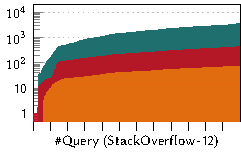
\includegraphics[scale=0.95]{plots/Experiment2-Stackoverflow12-Speed-Micro}
    \vspace{-0.45cm}
    \caption{Per-query Time Saved by {\sys} on the 1,190 \textsf{StackOverflow} Queries at Scale Factors 1 (left) and 12 (right).}
    \label{fig:stackoverflow_micro1}
    \vspace{-0.5cm}
\end{figure}


% TODO(Saeed): confirm that 38.7x uses the pooled library of 67 rules (also in Section 6.4); if not, state the rule set used.
% Saeed: yes, 38.7x (and the whole SOLEX column in the upper part of Table4) uses the pooled library; see the blue sentences in Workload Samples (Section 6.1) and below. Own rules give 12.7x and JOB rules 28.3x (Section 6.4). Caveat: 67 rules is exact for PostgreSQL; the DuckDB and MySQL runs predate four DSB-derived rules (63 rules).
\textbf{LLM Rewriter Comparison:} ReSequel rewrites each template with the LLM and applies the selected rewrite to its queries. {\sys} distills rewrites into rules that apply to any query they match. \blue{All {\sys} results in the upper part of Table~\ref{tbl:e2e} use the pooled library, the 67 distinct rules of all workloads.} On \textsf{Stats-CEB}, {\sys} reduces total time by $38.7\times$ versus ReSequel's $12.9\times$ on PostgreSQL, $60.5\times$ versus $1.8\times$ on MySQL, and $11.6\times$ versus $8.5\times$ on DuckDB. On \textsf{StackOverflow}, ReSequel's per-query geometric mean is comparable, but {\sys} wins in total time (Section~\ref{sec:exp:scalability}).

% Saeed: LearnedRewrite is not a LLM-based baseline
\textbf{(LLM) Rewrite Selector Comparison:} LearnedRewrite ($1.05$--$1.10\times$) and R-Bot ($1.03$--$1.04\times$) barely yield any improvements on \textsf{Stats-CEB}, because their rule libraries cannot express factorized aggregation. On \textsf{StackOverflow}, LearnedRewrite rewrites $62\%$ of the queries on PostgreSQL and DuckDB ($55\%$ on MySQL), but not the bottlenecks. Calcite's rules move a filter into a sub-select and re-type its predicate as \texttt{CAST(posttypeid AS INTEGER) = 1}, which hides the column from PostgreSQL's statistics and indexing. Its rewrites slow PostgreSQL down to $0.85\times$ at scale~1 and $0.28\times$ at scale~12, where $652$ of $1{,}190$ queries regress. LearnedRewrite searches its rules with MCTS, but no search finds a new transformation.

\subsection{Scalability}
\label{sec:exp:scalability}
The next experiments tests whether {\sys}'s gains hold as data and concurrency grow, and what the impact of reusing the host's engine is. We vary the \emph{data size} with \textsf{StackOverflow} at scale factors 1 and 12 on all three hosts (Table~\ref{tbl:e2e}, Figure~\ref{fig:stackoverflow_micro1}), as well as \emph{parallelism} with the \textsf{CEB} queries at scale factors 1--10, single- and multi-threaded, compared to BespokeOLAP (Figure~\ref{fig:ceb_micro0}).

% Saeed: 5, not 7, rules fire on the 1190 queries per stackoverflow_{1,12}
\textbf{Increasing Data Size:} The \textsf{StackOverflow} workload has a uniform shape. The typical query joins \textsf{Posts} and \textsf{Users}, left-joins two one-to-many child tables (\textsf{Comments}, \textsf{Votes}), groups per post, and keeps ten rows by \texttt{CreationDate}. The engine builds a cross product of comments and votes per post only to collapse it in the aggregate, and the \texttt{LIMIT} sits above the aggregate, where hosts do not push it down. \blue{Two of the five rules that fire address these bottlenecks.} A top-$k$ prefilter rule (200 queries) cuts the driving table to ten surviving rows before the fan-out joins. \texttt{JoinDecomposeTo}\allowbreak\texttt{Preaggregated}\allowbreak\texttt{Count} (334 queries) counts each fan-out branch in its own CTE and multiplies the counts, which removes the cross product. 
%
The margin \emph{grows} with increasing data size (see Table~\ref{tbl:e2e}): when going from scale~1 to scale~12, speedups increase from $1.82\times$ to $2.92\times$ on PostgreSQL and from $3.62\times$ to $12.58\times$ on MySQL, respectively. The work {\sys} removes grows faster than the data, while the remaining work is capped by the \texttt{LIMIT}. For a $12\times$ data increase, the unmodified hosts grow $26.5\times$ (PostgreSQL) and $19.6\times$ (MySQL), but only $16.4\times$ and $5.6\times$ under {\sys}. DuckDB already grows slower than the data ($8.5\times$), so the speedup stays flat at $1.65\times$.\shorten

\textbf{Sample-based Selection:} The \textsf{StackOverflow} 1,190 queries are covered by 60 templates in ReSequel, which rewrites almost all of these queries ($1{,}118$ on PostgreSQL, $1{,}186$ on MySQL). Its geometric mean is comparable ($2.79\times$ versus $2.42\times$ on PostgreSQL at scale~12), but {\sys} wins in total time, by $1.19\times$ on PostgreSQL and $2.95\times$ on MySQL. ReSequel times each candidate on a downsampled database, which keeps the query shape but not the cardinalities. Query~\#15112 is the clean case. ReSequel's pick replaces \texttt{COUNT}/\texttt{SUM} with \texttt{COUNT(DISTINCT $\cdot$)} but keeps the joins, which is cheap on the sample. At scale~12 it takes $714.2$\,s against the host's $394.0$\,s, while {\sys} removes the product and finishes in $4.0$\,s. At scale~12, ReSequel is slower than the host on 53 PostgreSQL and 41 MySQL queries, but on only four MySQL queries at scale~1.

\textbf{Negligible Regressions:} Figure~\ref{fig:stackoverflow_micro1} shows the time {\sys} saved per query. On PostgreSQL, regressions cost $0.04\%$ and $0.42\%$ of host time at scale~1 and~12, against savings of $45\%$ and $66\%$; on MySQL, $0.003\%$ and $0.05\%$ against $72\%$ and $92\%$. DuckDB is the only host where regressions are visible: $345$ and $378$ queries are slower, costing $5.0\%$ and $11.4\%$ against $44\%$ and $52\%$ saved. They share one pattern: when the group-by key is not the driving table's primary key, the top-$k$ rule falls back to a range bound that blocks a push-down DuckDB would otherwise do (query~\#15371, $6.0$\,s\,$\to$\,$32.3$\,s).

\textbf{Parallelism:} Figure~\ref{fig:ceb_micro0} compares DuckDB, {\sys} on DuckDB, and BespokeOLAP on the 16 \textsf{CEB} queries at scale factors 1--10 (five iterations, no buffer-pool cap). Scale factors are obtained by duplicating the \textsf{IMDB} tables with primary- and foreign-key renumbering, which preserves referential integrity and predicate selectivities. BespokeOLAP generates and compiles one physical implementation per query over Parquet inputs. Before the first query, it reads the Parquet files, ingests them, and preprocesses them into its layout, and it repeats these phases on every run.
% TODO(Saeed): NEW RUN, DuckDB load time for IMDB at scale factors 1 and 10; add it to SOLEX end-to-end times
%   and recompute 1.89-2.67x, 2.25x, and 2.05x.
% Saeed: no new run is possible here. DuckDB has no separate load phase to time: the queries run on a persistent database file (imdb_sf<N>.duckdb), DuckDB reads its pages on demand during query execution, and it does not report I/O time separately from CPU time. The measured SOLEX times therefore already include all of DuckDB's I/O, and 1.89-2.67x, 2.25x, and 2.05x stay as they are. Only the one-time import into the database file is outside these times; it is done once, not on every run.
With single-threaded execution, BespokeOLAP outperforms {\sys} at every scale factor (Figure~\ref{fig:ceb_micro0}, solid bars), and its query execution alone is the fastest: $15.0$\,s for all 16 queries at scale~1, against $25.1$\,s for {\sys}. This win costs \$303 and 10--30~hours of synthesis time (Section~\ref{sec:exp:generation}), plus the preparation phases on every run. With 32 threads (hatched bars), however, {\sys} on DuckDB gains $5.5\times$ at scale~1 and $7.8\times$ at scale~10, because the host parallelizes the rewritten plans. BespokeOLAP's query execution gains only $1.12$--$1.69\times$, and its end-to-end time $1.07$--$1.58\times$: loading and pre-processing take $63$--$73\%$ of each run, and multi-threading does not improve this pre-processing. End to end, {\sys} is faster at every scale factor, by $1.89$--$2.67\times$ ($2.25\times$ at scale~1, $2.05\times$ at scale~10). \blue{DuckDB has no separate load phase: it reads the persistent database file on demand during query execution, so the {\sys} times already include its I/O.} Here, the synthesized code performs well single-threaded, but does not exploit parallelism as effectively as a mature engine.

\textbf{Engine Layers Beyond Execution:} The synthesized engine runs on a fully materialized in-memory layout. Indexing, paged loading, and data skipping are not supported, so preparation grows with the data (blue segments in Figure~\ref{fig:ceb_micro0}): ingest time by $12.3\times$ and Parquet I/O by $8.6\times$ from scale~1 to~10. The generated engine also exposes only load, build, and query entry points~\cite{bespokeolap}\footnote{\url{https://github.com/DataManagementLab/BespokeOLAP}; its successor SynnoDB rejects writes by default or passes them to DuckDB in an unaccelerated manner.}, so it is read-only over a Parquet snapshot, and every data change repeats the preparation phases. With {\sys}, the host keeps handling updates, and the rules stay valid because they refer to no data values.\shorten 

\textbf{Host Bottleneck:} The \textsf{CEB} queries are unfiltered \texttt{COUNT(*)} joins over up to twelve tables. Their intermediate results reach roughly $800$\,GB, far beyond the server's $148$\,GB, so DuckDB spills them to disk, and parallelism increases spilling. {\sys} applies the factorized \texttt{COUNT(*)} decomposition of Section~\ref{sec:offline:distill}, so the query never forms the full join. Four queries (2a, 8a, 7a, 2b) account for $95\%$ of DuckDB's time at scale~1, and {\sys} runs them $310\times$, $62\times$, $41\times$, and $31\times$ faster, while the queries DuckDB already handles well stay at $0.9$--$1.4\times$. The rewritten plans keep their intermediates under $50$\,GB, without spilling and thus, parallelism helps. End to end this is $200\times$ over DuckDB at scale~1 and $31.4\times$ at scale~10. DuckDB completes all 16 queries only at scale~1, and fails up to 4 from scale~2 and 7--9 from scale~6 onward (labels in Figure~\ref{fig:ceb_micro0}). BespokeOLAP and {\sys} always complete all 16 queries.


\subsection{Rule Reuse on New Queries}
\label{sec:exp:generalization}
% TODO(Saeed): regenerate this figure (plots/Experiment2-JOB-to-Stats-CEB-Speed2-Micro) with the old panel (b) only.
\begin{figure}[!t]
    \centering
    \resizebox{.99\columnwidth}{!}{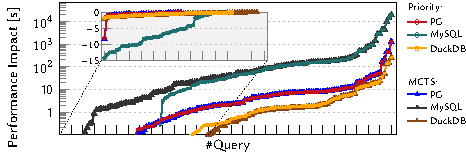
\includegraphics[scale=1]{plots/Experiment2-JOB-to-Stats-CEB-Speed2-Micro}}
   \vspace{-0.45cm}
    \caption{Per-query Time Saved on \textsf{Stats-CEB} by the Rules Distilled from \textsf{JOB}, Applied Unchanged.}
    \label{fig:gen_speed}
    \vspace{-0.3cm}
\end{figure}

We further evaluate the utility of distilled rules on new queries (requirement R3). Templates would only match identical structure.

% TODO(Saeed): from per-query logs, split StackOverflow at scale factor 1 (PostgreSQL) into the 51 sampled and 1,139 unseen
% Saeed: done, text updated. The sample is 8 queries (not 51), so the split is 8 sampled / 1,182 unseen: 1.64x (6.8 s -> 4.1 s) and 1.82x (742.9 s -> 408.3 s). A rule fires on all 1,182 unseen queries (a rule other than join commutation on 1,166, 98.6%). No LLM call on the 18,251 queries: the online rewriter has no LLM client.
\textbf{Unseen Queries of the Same Workload:} On \textsf{StackOverflow}, {\sys} distills rules from \blue{8} queries. On the \blue{1,182} unseen queries, it achieves \blue{$1.82\times$} speedup (\blue{at least one rule fires on every query}) on PostgreSQL \blue{at scale~1}, compared to \blue{$1.64\times$} on the \blue{8} sampled ones. \blue{The gain does not depend on the sample: \texttt{JoinDecomposeTo}\allowbreak\texttt{Preaggregated}\allowbreak\texttt{Count}, a rule of the pooled library that fires on none of the sampled queries, fires on 334 unseen ones and speeds them up by $2.23\times$.} On all \blue{18,251} queries, the rules reduce runtime by $1.43\times$ on DuckDB, \blue{with no additional LLM calls}.

% TODO(Saeed): which rules ran on CEB? Keep one option.
% Saeed: CEB ran the pooled library. 16 of 16 queries rewritten, 13 distinct rules fire. The JOB-only option is wrong: join_decompose_to_preaggregated_count (9 of 16 queries: 1a, 2a, 2b, 3a, 5a, 6a, 7a, 8a, 9b) is tagged stats_ceb not imdb.
\textbf{Unseen Workloads:} We take the rules distilled from \textsf{JOB}, without any modifications, and run them on \textsf{Stats-CEB}. The two workloads share no queries, tables, or schema, and no LLM is called. The total workload time reduces by $28.3\times$ on PostgreSQL, $6.6\times$ on MySQL, and $9.8\times$ on DuckDB (Table~\ref{tbl:e2e}); the per-query geometric means are $3.30\times$, $3.44\times$, and $1.59\times$. On PostgreSQL, the three rule sets compare as follows: the rules distilled from \textsf{Stats-CEB} itself give $12.7\times$, on par with ReSequel's $12.9\times$; the \textsf{JOB} rules give $28.3\times$; and \blue{the pooled library of 67 rules} gives $38.7\times$. What carries across is structure: the factorized \texttt{COUNT(*)} decompositions and foreign-key eliminations of Section~\ref{sec:offline:distill} do not depend on table names, constants, or number of joins.
%
On \textsf{CEB} (Section~\ref{sec:exp:scalability}), {\sys} uses \blue{the pooled library; no rule is distilled from \textsf{CEB} itself. All 16 queries are rewritten, and the factorized \texttt{COUNT(*)} decomposition behind the largest gains, a rule distilled from \textsf{Stats-CEB}, fires on 9 of them}.
%
Figure~\ref{fig:gen_speed} shows the per-query impact. The gains are substantial: the best query saves $1{,}278$\,s on PostgreSQL and $19{,}294$\,s on MySQL. The losses are many but small: 32, 44, and 53 of the 146 queries get slower, costing $0.7\%$, $0.4\%$, and $3.5\%$ of host time. The worst single loss on any engine is $14.3$\,s.

% TODO(Saeed): fill the coverage range after the coverage column of Table 3 is filled.
\textbf{Coverage:} \blue{Across all workloads, at least one rule fires on $50.0$--$100\%$ of queries, which account for $39.0$--$100\%$ of the host's time; only \textsf{TPC-H} and full \textsf{StackOverflow} are below $90\%$ (Table~\ref{tbl:datasets}).}


% TODO(Saeed): fill SOLEX and ReSequel rows from the logs; $ at Gemini-3.1-pro prices.
\begin{table}[!t]
\centering
\small
\caption{Cost to Specialize. \$ Uses Each System's Model Price (Gemini-3.1-pro; BespokeOLAP: \blue{Claude Sonnet 4.7}).}
\label{tbl:cost}
\vspace{-0.3cm}
\setlength{\tabcolsep}{3pt}
\begin{tabular}{llrrrr}
\toprule
\textbf{System} & \textbf{Workload}      & \textbf{LLM calls}   & \textbf{Tokens} & \textbf{\$} & \textbf{Time} \\ \midrule
{\sys}          & \textsf{Stats-CEB}     & 66                   & $0.60$\,M       & $3.05$      & $6.0$\,min \\
                & \textsf{CEB} (16)      & 0                    & 0               & $0$         & 0 \\
                & \textsf{StackOverflow} & 33                   & $0.25$\,M       & $1.27$      & $5.7$\,min \\
                & All nine               & 175                  & $1.60$\,M       & $8.72$      & $19.6$\,min \\ \midrule
ReSequel        & \textsf{Stats-CEB}     & 146                  & $1.27$\,M       & $10.30$     & $2.2$\,h \\
                & \textsf{StackOverflow} & 60                   & $0.73$\,M       & $5.87$      & $1.2$\,h \\ \midrule
BespokeOLAP     & \textsf{CEB} (16)      & \blue{$2{,}372$} & \blue{${\approx}160$\,M} & $303.25$    & 10--30\,h \\
\bottomrule
\end{tabular}
\vspace{-0.4cm}
\end{table}

\begin{figure}[!t]
    \centering
    \resizebox{.99\columnwidth}{!}{
    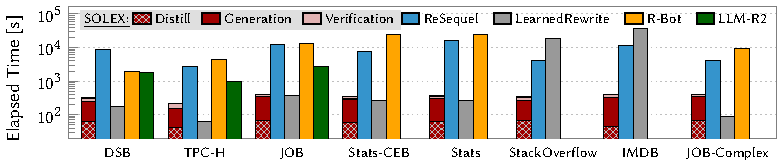
\includegraphics[scale=0.97]{plots/Experiment0-Quantization}}
    \vspace{-0.35cm}
    \caption{Rewriting Time per Workload (PostgreSQL): {\sys}'s Offline Phases Take Less than LLM Rewriters.}
    \label{fig:rewrite_time}
    \vspace{-0.55cm}
\end{figure}


\subsection{Cost of Specialization}
\label{sec:exp:generation}
We now substantiate the cost claims of Table~\ref{tab:intro-landscape}: {\sys} calls the LLM offline on sampled queries, and rewrites online without LLM calls. Table~\ref{tbl:cost} compares costs of {\sys}, ReSequel, and BespokeOLAP.

% TODO(Saeed): online rewrite latency (median, max) over all nine workloads; current values are StackOverflow only.
% Saeed: done, PostgreSQL for all workloads and DuckDB for CEB. Median / max per workload in ms: TPC-H 2 / 186, DSB 6 / 831, Stats 33 / 331, Stats-CEB 33 / 339, JOB 109 / 212, JOB-Complex 124 / 259, IMDB Full 10 / 377, CEB 338 / 525, StackOverflow (1,190) 1 / 110, StackOverflow (18k) 31 / 376. The old 1 ms / 97 ms were StackOverflow (1,190) only.
\textbf{{\sys}:} The LLM cost grows with the number of rules {\sys} generates per workload. The 125 rules reduce to 67 distinct ones after cross-workload deduplication, so a later workload pays only for its new rules, and reusing rules costs no LLM call (Section~\ref{sec:exp:generalization}). Figure~\ref{fig:rewrite_time} breaks the offline time into its phases: \emph{Distill} (sample selection and rule extraction), \emph{Generate} (C++ code synthesis), and \emph{Verify} (the verification stages), in log scale. 
\blue{Online rewriting takes a median of $1$--$338$\,ms per query depending on the workload, and at most $831$\,ms, without any additional LLM calls.}

% TODO(Saeed): number of templates the 18,251 StackOverflow queries form under ReSequel's templatization.
% Saeed: all templates= 16114, so the new templates = 16114 - 60 = 16054
\textbf{ReSequel:} ReSequel calls the LLM once per template. On \textsf{StackOverflow}, we run it on its 60 templates, which cover 1,190 of the 18,251 queries; the rest would need \blue{$16{,}054$} new templates, one LLM call each. On \textsf{TPC-H}, \textsf{DSB}, and \textsf{Stats-CEB}, every query is its own template~\cite{resequel}. R-Bot and LLM-R2 call the LLM for every query.

\textbf{BespokeOLAP:} Synthesizing the engine for the 16 \textsf{CEB} queries costs $\$303.25$ over roughly $15{,}000$ agent turns~\cite{bespokeolap}, of which $\$259.26$ is spent in per-query optimization stages. Synthesis takes $10$--$30$ hours, because these stages run serially, and it must be repeated when the workload changes. Both price and time grow with the number of templates: at $\$16.20$ and $0.6$--$1.9$\,h per template, the 60 \textsf{StackOverflow} templates would cost about $\$970$ and $36$--$114$\,h.

%%%%%%%%%%%%%%%%%%%%%%%%%%%%%%%%%%%%%%%%%%%%%%%%%%%

\subsection{Rule Verification}
\label{sec:exp:verification}
The final experiment tests requirement R1: the correctness of rules.

% TODO(Saeed): from the generation logs, per workload: number of candidate rules, proven by the formal check,
%   admitted by the result-equivalence test, rejected, and average retries. Totals go here; the per-workload table goes to the appendix. 

\textbf{Rule Verdicts:} \blue{All 67 rules in the library fired on the evaluated queries. For 37 of them, a formal verifier, SQLSolver, proved at least one rewritten query equivalent to its original. The remaining 30 rules relied on the result-equivalence test alone (Table~\ref{tbl:rule_verdicts} in the appendix). An admitted rule averaged $1.9$ fix iterations (at most 7).}

% TODO(Saeed): NEW RUN (most important). For every evaluated query (including JOB rules on Stats-CEB, and CEB),
%   compare order-insensitive result hashes of the original and the rewrite on DuckDB, full data. Report the number of matches.
%   If any mismatch, report it; do not hide it.
% Saeed: done. I ran the final rewritten queries on the original (full) datasets and compared their results with those of the original queries. For all nine workloads, I found no mismatch.

% TODO(Saeed): NEW RUN (seconds). Re-run the result-equivalence test with the JOB rules on the Stats-CEB samples.
% Saeed: done. I ran the Stats-CEB queries rewritten with the JOB rules on the full Stats-CEB data and compared their results with those of the original queries. I found no mismatch.
\textbf{Full-data Check.} \blue{For every rewritten query of all workloads except \textsf{StackOverflow} (18,251), we compare order-insensitive hashes of the results of the original query and its rewrite on the full data (DuckDB). All $16{,}516$ rewrites return the same result.} \blue{The \textsf{JOB} rules also pass the result-equivalence test on the \textsf{Stats-CEB} samples before we apply them in Section~\ref{sec:exp:generalization}.}

\begin{figure}[!t]
    \centering
    \resizebox{.99\columnwidth}{!}{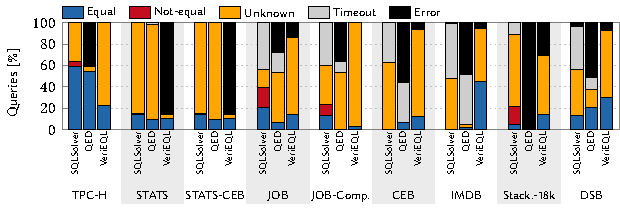
\includegraphics[scale=1]{plots/Experiment1-Verify-Baselines}}
    \vspace{-0.25cm}
    \caption{Verdicts of Three Standalone Equivalence Verifiers on {\sys}'s Final Rewrites (\% per Workload, $200$\,s per Pair): Query-level Checks Leave Most Pairs Undecided.}
    \label{fig:verify_baselines}
    \vspace{-0.35cm}
\end{figure}

%MB TODO: why does the large veryification runtime per query pair not show up in Figure 8 (yes, it's log scale but 1500 hours should show up)
% Saeed: they are two different measurements. The 1,599 CPU-hours are the three standalone verifiers run on every one of the 32,423 query pairs (Figure fig:verify_baselines): 32,423 x (57.9 + 45.8 + 73.8) s. SOLEX never runs this; it is the baseline this paragraph argues against. The Verify segment of Figure fig:rewrite_time is SOLEX's own per-rule verification on the sampled queries (SMT_time + test_suite + sample_test), 63--87 s per workload. Clarified in the text below.

\textbf{Verify Rules not Queries:} We run SQLSolver, QED, and VeriEQL as-they-are over all $32{,}423$ pairs of original and rewritten queries from the nine workloads. Each pair covers the composition of all rules that fire on the query. Figure~\ref{fig:verify_baselines} shows the verdicts. Query-level verification is both incomplete and costly. VeriEQL finds $8{,}778$ pairs ($27.1\%$) equal up to its bound, SQLSolver proves $954$ ($2.9\%$), and QED $372$ ($1.1\%$). Even with the best answer of any tool, $63.5\%$ of the pairs get no answer. QED cannot parse $76.9\%$ of the pairs, including all $18{,}251$ \textsf{StackOverflow} ones; SQLSolver times out on $28.0\%$. What the tools decide follows how complex the SQL is: SQLSolver proves $59.1\%$ of \textsf{TPC-H}'s 22 queries but none of the $13{,}646$ \textsf{IMDB Full} ones. The average time per pair is $57.9$\,s (VeriEQL), $45.8$\,s (QED), and $73.8$\,s (SQLSolver), $1{,}599$ CPU-hours in total.
{\sys} therefore verifies each \emph{rule} once, when it is admitted (Definition~\ref{def:verification}). \blue{This is the \emph{Verify} phase of Figure~\ref{fig:rewrite_time}, which takes only $63$--$87$\,s per workload because it runs on the sampled queries, not on every query pair.} The formal check covers the rule on its source query, and the result-equivalence test covers rules the solver leaves undecided, together with the rules already admitted. Later queries reuse this verdict instead of a new proof.


\subsection{Impact of Rule Ordering and Engines}
\label{sec:exp:discussion}
Two questions cut across the experiments: when does the \emph{order} in which rules fire change the outcome, and when does a rewrite pay off on the host engine? Both are workload- and engine-dependent.

\textbf{When Rule Ordering Matters:} {\sys} applies rules in the priority order the LLM assigns at generation time, which is deterministic, or in an order found by MCTS, guided by the cardinality estimator of Section~\ref{sec:online:cost} and adopted only when its estimated cost is at least $5\%$ below the priority plan's.
\begin{itemize}
\item \emph{Search helps when rules compete at a plan node.} Where a workload mixes aggregation, multi-block subqueries, and long join chains, a decomposition rule and a push-down rule are often applicable at the same node, and whichever fires first forecloses the other. On \textsf{DSB}, search brings $1.10\times$ over priority order on DuckDB; on \textsf{TPC-H} only $1.04\times$.
\item \emph{Search is irrelevant when a single rewrite dominates.} On \textsf{JOB-Complex} and on rules transferred from \textsf{JOB} to \textsf{Stats-CEB}, one semijoin lift or factorized aggregation dominate the runtime benefit. MCTS yields only $1\%$ over priority order.
\item \emph{Search hurts if the cost proxy is inaccurate.} The estimator assumes uniform value distributions, independent predicates, and containment of join keys. On \textsf{DSB}'s skewed fact tables, it predicts $88\%$ cost reduction but realizes only $1.10\times$. It also cannot see the physical plans: e.g., on PostgreSQL, a count decomposition runs as a per-row subplan, and \textsf{query58} degrades from $228$\,ms to $>21$ minutes. On MySQL, \textsf{Stats-CEB}, MCTS yields only $3.8\times$ compared to priority order's $60.5\times$. We therefore default to priority order, and adopt search only under the rule of Section~\ref{sec:online:mcts}.
\end{itemize}

% TODO(Saeed): DuckDB speedup on Stats-CEB: 11.6x (Section 6.2) or 7.16x (earlier draft of this paragraph)? Keep one, and explain the other if both are valid.
% Saeed: keep 11.6x; 7.16x is not valid. 11.6x is the current 5-rep run (host 952.0 s -> 82.2 s, Table4).
\textbf{Rule Impact Depends on the Execution Engine:} The speedup of a rewrite depends on what the host optimizer already does. PostgreSQL and MySQL lack rewrites for several {\sys} transformations, so the same rewrites gain more: \textsf{Stats} improves $26.9\times$ on PostgreSQL and $29.2\times$ on MySQL versus $11.3\times$ on DuckDB, and three \textsf{Stats-CEB} queries drop from >4 hours to <4 seconds on MySQL. DuckDB's optimizer already performs many of these transformations. On \textsf{TPC-H}, the distilled rules are mostly canonicalization and push-downs, so the impact is limited (\blue{$1.11\times$}). On \textsf{Stats-CEB}, the median query is neutral (\blue{$0.86\times$}) and the gain ($11.6\times$, Table~\ref{tbl:e2e}) comes from a few large \texttt{COUNT(*)} star joins. On DuckDB, {\sys}'s value comes from a few rules outside its repertoire, such as factorized aggregation and foreign-key elimination. The plans with the biggest gains are dependent on accurate cost estimates though.